\documentclass[12pt]{article}
\usepackage{listings}
\usepackage{amsmath}
\usepackage[pdftex]{graphicx}
\usepackage{fancyvrb}
\usepackage{chapterbib}
\usepackage{hyperref}
\usepackage{wrapfig}

\pdfcompresslevel=9
\DeclareGraphicsExtensions{{.png},{.pdf},{.jpg},{jpeg}}
\graphicspath{ {../figures/}}
\usepackage{color}

%__________________________________
% new commands for all sections --- !!!! FIXME: This should be pulled in from
% user_guide.tex... not sure how to do this !!!!
\newcommand{\TT}[1]{\tt{#1} \normalfont}

\begin{document}

\title{Uintah Installation Guide}

\author{Jim Guilkey, Todd Harman, Justin Luitjens, John Schmidt,
  \\ Jeremy Thornock,
  J. Davison de St. Germain, Siddharth Shankar, \\
  Joseph Peterson,  
  Carson Brownlee}

\date{Version 1.1}

\maketitle



\newpage

\tableofcontents

\newpage

\section{Overview of Uintah} \label{sec:overview}

The \textbf{Uintah} library is composed of several executables and a
generic library framework for solving PDEs on structured AMR grids on
large parallel supercomputers. The \textbf{\emph{VisIt}} and
\textbf{\emph{Teem}} applications are used to visualize data generated
from \textbf{Uintah}.

\subsection{Obtaining the Code}
Uintah can be obtained either as a compressed tarball from
\url{http://www.uintah.utah.edu/trac/chrome/site/uintah.tar.gz} or by using
Subversion (SVN) to download the latest source code:

\begin{verbatim}
svn co https://gforge.sci.utah.edu/svn/uintah/trunk uintah
\end{verbatim}

The above command checks out the \textbf{Uintah} source tree and
installs it into a directory called uintah in the users home
directory.


\section{Installation Overview}

If \textbf{Uintah} is installed on a workstation and one wants to
visualize the data generated, the visualization tools
\textbf{\emph{VisIt}} and \textbf{\emph{Teem}} should be installed
prior to installation of \textbf{Uintah}.  The configure script used by
\textbf{Uintah} depends on the presence of these libraries.

However, if \textbf{Uintah} is installed on a supercomputer, the
visualization tools do not need to be installed prior to installation
of \textbf{Uintah}.

The installation procedure follows the basic outline:

\begin{enumerate}

\item Install basic dependencies: MPI, Blas, Lapack, Hypre, PETSc, \emph{etc}.

\item Install visualization tools (optional if installing on a supercomputer)

\item Configure Uintah

\item Compile Uintah


\end{enumerate}


\section{Generic Library Dependencies}

\textbf{Uintah} depends on several different libraries that are commonly
available or easily installable on various Linux or Unix like OS
distributions.  

Required libraries:
\begin{itemize}
\item mpi (OpenMpi, Mpich, or LAM or a vendor supplied mpi library)
\item blas
\item lapack
\item make
\item libxml2-devel
\item zlib-devel
\item c++
\item fortran
\item subversion
\item ccmake

\end{itemize}

Useful libraries:
\begin{itemize}
\item Hypre v2.4 (\url{https://computation.llnl.gov/casc/hypre/software.html})
\item PETSc v3.0 (\url{http://www.mcs.anl.gov/petsc/petsc-as/download/index.html})
\end{itemize}

Note, Uintah recently upgraded from using Hypre v2.0 and PETSc
v2.3.3.  (July 22, 2009)

\section{OS Version Dependencies}

\subsection{Debian Dependencies}
\label{sec:debian_dependencies}
The \textbf{Gnu/Debian} OS \url{http://www.debian.org} offers the vast majority of libraries necessary for
installing \textbf{Uintah} with the exception of VisIt and Teem.

Installing the following libraries will ensure that all dependencies
required for \textbf{Uintah} are satisfied: 

\begin{verbatim} 
sudo aptitude install subversion libhypre-dev petsc-dev \ 
libxml2-dev zlib1g-dev liblapack-dev cmake libglew1.5-dev \
libglui-dev libxmu-dev
\end{verbatim}

Once these libraries are installed, Teem and VisIt can be installed
followed by installation of \textbf{Uintah}.

\subsection{Fedora Core 9 Dependencies}

\textbf{Fedora Core 9} \url{http://fedoraproject.org/} offers all the
dependencies except for PETSc and hypre.  Install the following
libraries:
\begin{verbatim}
sudo yum install openmpi-devel openmpi-libs lapack-devel \
gcc-gfortran blas-devel gcc-c++ libxml2-devel subversion \ 
make tar diffutils
\end{verbatim}

\subsubsection{MPI issues} 
\label{sec:mpi}

The OpenMPI library that is installed with \textbf{Fedora Core 9}
needs to have a 'helper' directory set up with symbolic links assigned
so that during the \emph{configure} of \textbf{Uintah} can find the
location of specific include files and shared libraries.

Execute the following as root:

\begin{Verbatim}
mkdir /usr/local/openmpi
cd /usr/local/openmpi
ln -s /usr/include/openmpi/1.2.4-gcc include
ln -s /usr/lib64/openmpi/1.2.4-gcc lib
\end{Verbatim}

In the event that soft linking the libraries does not work, it may be
required to actually copy the shared library to a suitable location
and then performing the soft linking as in:

\begin{Verbatim}
cp /full/path/to/openmpi/lib/libmpi.so.0.0.0 .
ln -s libmpi.so.0.0.0 libmpi.so
\end{Verbatim}


\subsection{CentOS 5 Dependencies}

\textbf{CentOS 5} \url{http://www.centos.org/} is similar to \textbf{Fedora
Core 9} however, it does not provide an OpenMpi rpm.  A src.rpm can be
downloaded from \url{http://www.open-mpi.org:80/software/ompi/v1.3/}
and installed via rpmbuild

\begin{Verbatim}
rpmbuild --rebuild --define 'dist .centos5' openmpi-1.3.1-1.src.rpm
rpm -i openmpi-1.3.1-1.*.rpm
\end{Verbatim}
The location of the rpm is likely to be found in
/usr/src/redhat/RPMS/ARCH where ARCH is either i386 or x86\_64.

Once MPI has been built, the other libraries can be installed:
\begin{verbatim}
sudo yum install lapack-devel gcc-gfortran blas-devel gcc-c++ \
libxml2-devel subversion make tar diffutils
\end{verbatim}


\section{PETSc Installation}

PETSc can be installed by executing the following simplified
instructions.  Please refer to the PETSc website for comprehensive
installation instructions if you encounter any difficulties.

Download petsc-3.0.0 from
\url{http://www.mcs.anl.gov/petsc/petsc-as/download/index.html}

The following configure script assumes the location of MPI is in
/usr/local/openmpi using the Fedora Core 9 OS.  For other OS
distributions, the location of the MPI libraries may be found
automatically.

\begin{Verbatim}
tar zxf petsc-3.0.0.tar.gz
cd petsc-3.0.0-p7

./config/configure.py --with-shared --with-debugging=0 \ 
--with-mpi-dir=/usr/local/openmpi/ --prefix=/usr/local/petsc

make all
make install
\end{Verbatim}

\section{Hypre Installation}

Hypre can be installed by executing the following simplified
instructions, however, if you encounter problems please refer to the
hypre website for troubleshooting.

Download hypre-2.4 from
\url{https://computation.llnl.gov/casc/hypre/download/hypre-2.4.0b\_reg.html}

If installing hypre on a 64bit platform, hypre must be modified to add
the -fPIC compile option.  After unpacking the hypre tar file, edit
the Makefile in \tt hypre-2.4.0/src/lapack \normalfont and add the
-fPIC to line 128.  It should look like the following:

\begin{verbatim}
${CC} -c -fPIC dlamch.c
\end{verbatim}

Depending on the location of the MPI libraries, i.e. location of mpi.h
and libmpi.so, the configure line for hypre should look like this:
\begin{verbatim}
cd hypre-2.4.0/src

./configure \
  --enable-shared \
  --with-MPI-include=/usr/local/openmpi/include \
  --with-MPI-lib-dirs=/usr/local/openmpi/lib \
  --with-MPI-libs="mpi pmpi util" \
  --prefix=/usr/local/ CFLAGS=-DMPIPP_H CXXFLAGS=-DMPIPP_H

make
make install
\end{verbatim}

\emph{Note, under Mac OSX, Hypre does not handle the "--enable-shared" configure
  flag correctly.}

\section{Installing Visualization Tools}

Visualization of \textbf{Uintah} data is currently possible using
\textbf{\emph{VisIt}}. The VisIt package from LLNL is general purpose
visualization software that offers all of the usual capabilities for
rendering scientific data.  It is still developed and maintained by
LLNL staff, and its interface to \textbf{Uintah} data is supported by
the Uintah team.

% Manta offers volume rendering and particle visualization based on
% parallel (shared memory) ray tracing techniques.  While the
% capabilities of Manta are more limited, it is a fast way to
% interactively interrogate reasonably large datasets, provided the user
% has access to a reasonable shared memory resource, (e.g. an 8 core
% desktop system).

\subsection{Teem Installation}
\label{subsec:teem}


Download Teem from
\url{http://teem.sourceforge.net/download/index.html}.  Teem uses
CMake to configure the build system. Installation instructions for
Teem are found at \url{http://teem.sourceforge.net/build.html}.  Simplified
instructions are as follows:

\begin{verbatim}
tar zxf teem-1.10.0-src.tar.gz
cd teem-1.10.0-src/
mkdir teem-build
cd teem-build
ccmake ../
\end{verbatim}

Use the arrow keys to scroll down to the fourth line
BUILD\_SHARED\_LIBS and press the return key to toggle the ON flag.

\begin{verbatim}
Press the 'c' key

Press the 'g' key

make
make install
\end{verbatim}
The Teem libraries and include files will be install in /usr/local
hierarchy.  If you have a /usr/local/lib64 directory please make a
symbolic link to the libteem.so found in /usr/local/lib, i.e.

\begin{verbatim}
cd /usr/local/lib64
ln -s ../lib/libteem.so libteem.so
\end{verbatim}

\subsection{VisIt Installation}

\subsubsection{Client/Server}
\label{subsec:ClientServer}

You will most likely want to install a VisIt server on a
multiprocessor machine. This requires you to build the server from
source (as it is needed to compile the UDA reading plugin). You can
then install any client on your local machine and attach to the
server.

\subsubsection{Caveats}
\label{subsec:VisIt_Caveats}
\begin{itemize}
\item The official release of VisIt is version 1.12.  However, a
  number of changes have been made to the VisIt trunk to support
  Uintah data. To get these changes it is necessary to install version
  2.0.  Make sure to use the v2.0 instructions below if this is the
  version you wish to use.
\item Before you install VisIt, a number of dependency files are
  required.  These include X11, GL, GLU, GLX, and libz libraries (it is possible
  that you will find these libraries in the following rpms:
  libx11-dev, libxext-dev, libxt-dev, libglu, zlib-dev -- notice that
  most of these are the 'development' rpm).  You can either install
  these directly and hope you get them right, or you can install the
  files listed here~\ref{sec:debian_dependencies} (which will
  hopefully pull in all the libraries that you need).
\item MPI must be installed and the MPI compilers (mpicc, etc) must be
  in your path.
\item The VisIt executable is not relocatable once it is built, so
  make sure you specify the correct installation location in the
  beginning.
\item Building VisIt from scratch can take a while.  As mentioned
  below, you can \begin{verbatim}tail -f build_visit_log\end{verbatim} to watch the progress.

\end{itemize}

\subsubsection{Prebuilt binaries}
\label{subsec:PrebuiltBinaries}

Warning, most of these binaries are for v1.12... If you need v2.x, then you
will need to build from source.

If you have a system that matches the prebuilt binaries, found at
\url{https://wci.llnl.gov/codes/visit/executables.html}, you may want
to try one. In most cases you will want to build your own
binaries. There are currently no universal binaries available for Mac
OS X 10.5 (leopard).

\subsubsection{Building Version 2.0}
\label{subsec:VisItVersion2_Build}

The VisIt source code (the 'trunk') can be checked out from the
repository maintained at NERSC:

\begin{verbatim}
mkdir ``new_visit_dir''
cd ``new_visit_dir'' 
svn co http://portal.nersc.gov/svn/visit/trunk/ .
\end{verbatim}

Create a new 'build' directory inside ''new\_visit\_dir'':

\begin{verbatim}
mkdir build
cd build
\end{verbatim}

Copy the 'build\_visit' script into the build directory:

\begin{verbatim}
cp ../src/svn_bin/build_visit .
chmod +x build_visit
\end{verbatim}

Copy the dependencies into the build directory. The build\_visit script
normally fails when trying to download the dependencies.  Copying them
skips the downloading phase.

\begin{verbatim}
cp ../third_party/*.tar.gz .
\end{verbatim}

Run the 'build\_visit' script (in order to just build the dependencies):

\begin{verbatim}
./build_visit --makeflags -j# --no-visit
\end{verbatim}

Replace '\#' with the number of processors you want to use.

This would launch the normal dialog window, where you should select
the ''Parallel'' option.  (Use the arrow keys and the space bar.)

At the end of this process, a config file would be generated. It will
be named ``your\_machine\_name''.conf. Copy this into the
''../src/config-site'' folder,

\begin{verbatim}
cp ``your_machine_name''.conf ../src/config-site
\end{verbatim}

Change directory to the ''src'' folder and run configure,

\begin{verbatim}
cd ../src
./configure --enable-parallel
\end{verbatim}

Before you run configure, check your ``your\_machine\_name''.conf
file: Both The CFLAGS and the CXXFLAGS compiler flags should have the
'-I/<your\_open\_mpi\_path>/include' set. If not please set them on the
''configure'' command, i.e. something like:

\begin{verbatim}
./configure --enable-parallel CXXFLAGS=-I/usr/local/openmpi/include CFLAGS=-I/usr/local/openmpi
\end{verbatim}

Note, you can alternatively set these in your .conf file.

After the configure process is over, run make:  (See below for
information on common errors that occur during the 'make' process.)

\begin{verbatim}
make -j#
\end{verbatim}

where '\#' is the number of processors to use while building.

As usual, cross your fingers. If everything goes fine, you can find
the visit executable in the ''bin'' folder, which is inside the
''src'' folder.

P.S.: When you run 'make', you may encounter this error:

\begin{verbatim}
error: `VERSION' was not declared in this scope
\end{verbatim}

If so, add in the line:

\begin{verbatim}
#define VERSION ``2.0.0''
\end{verbatim}

to the file, ./include/visit-config.h and run make again.

\subsubsection{Using the build script (Version 1.11) }
\label{subsec:UsingTheBuildScript}

Note, the following instructions are slightly different from the instructions
for building version 2.x:

We recommend that you first try the visit build script (WARNING, make
sure you get the must recent version of this script. The build script
must correspond to the version of VisIt you wish to install. The
latest version is 1.11.2). This is a link to the script,
\url{https://wci.llnl.gov/codes/visit/1.11.2/build\_visit}.

You can also use the following command on the terminal (from most
Linux boxes), to download the file directly,

\begin{verbatim}
wget https://wci.llnl.gov/codes/visit/1.11.2/build_visit
chmod +x build_visit
\end{verbatim}
The chmod is used to set execute permissions on the file.

\emph{build\_visit} is a bash build script that downloads and builds VisIt as
well as all of the necessary third party libraries. The script makes
use of the dialog program which allows you to customize your build.

Once you have the script, you would need to execute the following on
the terminal,

\begin{verbatim}
./build_visit --makeflags '-j#'
\end{verbatim}
where '\#' is the number of processors to use, while building VisIt.

This would launch a dialog window and would require you to select some
options (using the Space bar). You should select the 'Parallel'
option, if you wish to have a parallel build of the engine. Once you
have selected the parallel option, you may be required to specify the
path to the include and lib directories of your MPI installation.

The process of building VisIt may be slow and it may appear that
nothing is happening. To verify the build script is not hanging, open
another terminal and tail the file build\_visit\_log .

\begin{verbatim}
tail -f build_visit_log
\end{verbatim}

\normalfont  
\subsubsection{Parallel OS X build}
\label{sec:ParallelOSXBuild}

A full parallel OS X build can be built using the instructions above,
but it will fail when it tries to build the visit executable (the last
stage of the script). When it fails, you will need to follow the
instructions for building in parallel on a Mac.

\url{http://visitusers.org/index.php?title=Building_in_parallel_on_a_Mac}

  
Note particularly the changes that need to be made in the file, 

\begin{verbatim}
<path\_to\_visit>/visit1.11.2/src/config-site/<your_machine_name>.conf
\end{verbatim}

\normalfont Once you make these edits, you can then finish building VisIt by typing make in the \tt <path\_to\_visit>/visit1.11.2/src \normalfont directory.  

\subsubsection{When the build script fails}
\label{sec:WhenTheBuildsSriptFails}

Sometimes the build script doesn't work depending on your
installation. When this happens, you may be forced to build everything
by hand. The instructions for doing this are carefully outlined in the
VisIt Build Notes file,

\begin{verbatim}
https://wci.llnl.gov/codes/visit/1.11.2/BUILD_NOTES
\end{verbatim}

\subsubsection{VisIt executable}
\label{sec:VisItExecutable}

After a successful build, the executable will be placed in,

\begin{verbatim}
<path\to\visit>/visit1.11.2/src/bin
\end{verbatim}

\subsubsection{Building and installing the UDA reader plugin}
\label{sec:BuildingAndInstallingUDAPlugin}

Add the following arguments to the \textbf{Uintah} configure line,

\begin{verbatim}
--with-visit=/path/to/visit 
--with-teem=/path/to/teem
\end{verbatim}

For example,

\begin{verbatim}
--with-teem=/usr/sci/projects/Manta/Thirdparty/Linux/gcc-4.1.2-64bit/teem \
--with-visit=/home/csafe/dav/VisIt/blaze/visit1.11.2 \
\end{verbatim}

Note, the \tt visit1.11.2 \normalfont directory you point at should
have \tt data\normalfont , and \tt src \normalfont sub-directories;
and the \tt teem \normalfont directory should have \tt bin\normalfont
, \tt include\normalfont , and \tt lib \normalfont sub-directories.

\subsubsection{How it works}
By specifying the above configure arguments (to the \textbf{Uintah}
configure), \textbf{Uintah} will automatically build a VisIt plugin
(when you type "make"). The plugin will be placed in (a sub-directory
of) \textasciitilde/.visit. When VisIt is run, it will find the plugin
and allow for reading UDA's.

\subsubsection{Remote visualization}
In order to read data on a remote machine, you will need to have a
version of VisIt and the UDA reader plugin installed on that
machine. You will also need to make sure that the VisIt executable is
in your path. You may need to edit your shell's .rc file so that the
path to VisIt is included in your shell's PATH variable.

NOTE: The version of VisIt installed on your local desktop and the
remote machine should be the same.

\subsubsection{Host Profile}
Next you will want to set up a Host Profile for your remote
machine. Select 'Host Profiles' from the 'Options' menu and set up a
new profile as shown in figure ~\ref{VisItHostProfile}.


\begin{wrapfigure}{r}{100mm}

%\begin{figure}
  \begin{center}
  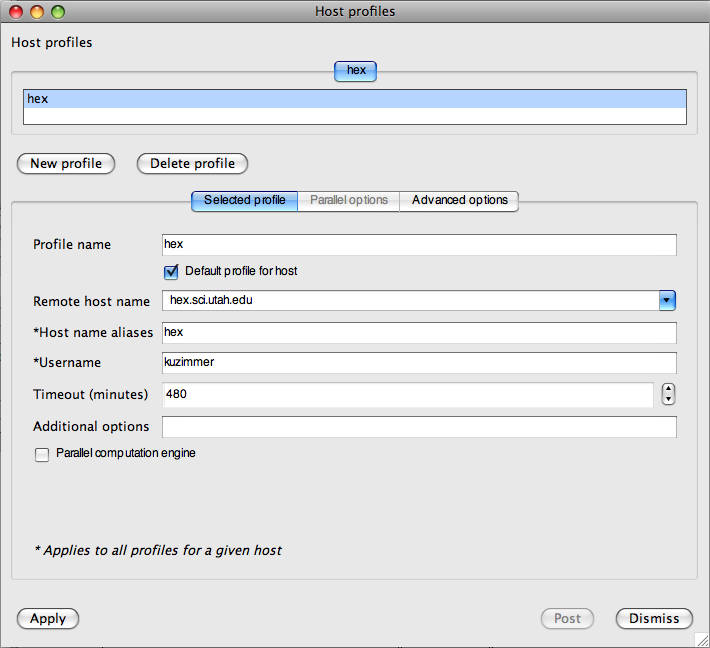
\includegraphics[scale=0.20]{VisItHostProfile.png}
  \end{center}
  \caption{Setting up Host Profile}
  \label{VisItHostProfile}
%\end{figure}

\end{wrapfigure}


After filling in the remote machine information, select the 'Advanced
options' tab, then 'Networking' and check the 'Tunnel data connections
through SSH' option. This is illustrated in
figure~\ref{VisItHostProfileAdv}. Click on 'Apply' and then do a 'Save
Settings' in the 'Options' menu on the gui.

\begin{wrapfigure}{r}{100mm}

%\begin{figure}
  \center 
  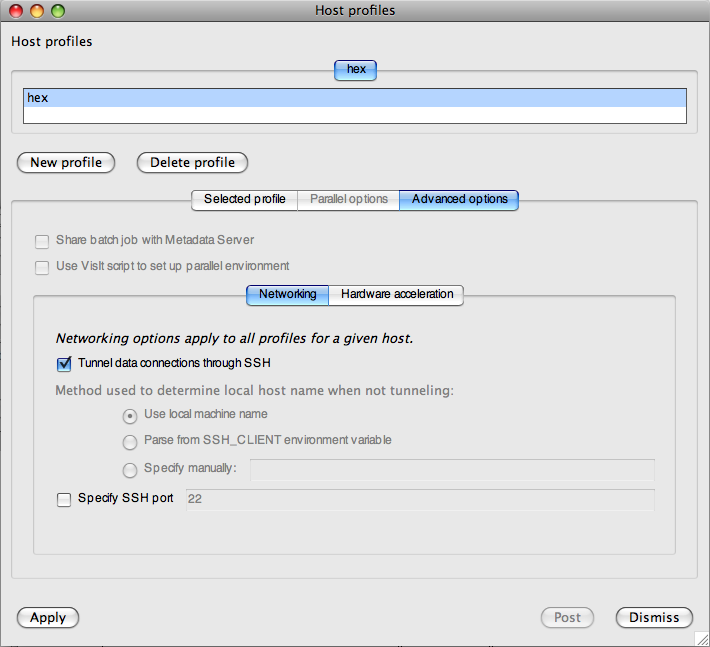
\includegraphics[scale=0.20]{VisItHostProfileAdv.png}
  \caption{Setting up advanced options}
  \label{VisItHostProfileAdv}
%\end{figure}

\end{wrapfigure}

For the remote visualization option to work, you must have ports 5600
- 5609 open. You can try this by running the following on your local
desktop (on Linux distributions),

\begin{verbatim}


traceroute -p 560[0-9] <remote machine>
\end{verbatim}

If the tunneling option doesn't works, try the option as shown in
figure~\ref{VisItHostProfileAdv2}.


\begin{wrapfigure}{r}{100mm}

%\begin{figure}
  \center
  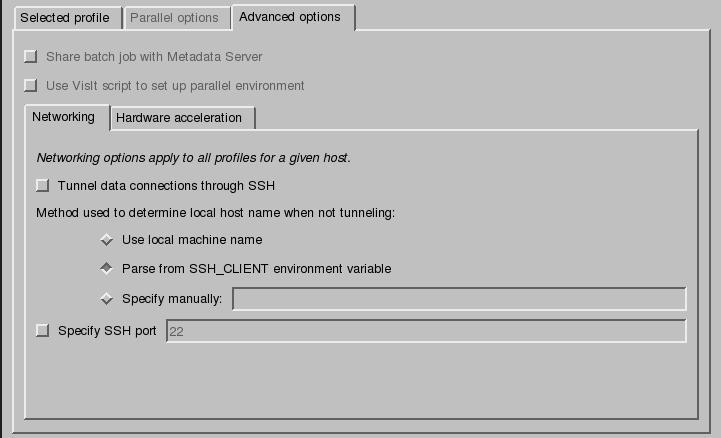
\includegraphics[scale=0.20]{VisItHostProfileAdv2.png}
  \caption{Setting up advanced options}
  \label{VisItHostProfileAdv2}
%\end{figure}

\end{wrapfigure}

Now you should be able select 'Open' from VisIt's 'File' menu. After
selecting your host from the host entry list, you will be prompted for
a password on the remote machine (unless you have set up passwordless
ssh access).

Once the ssh login has completed, you should see the directory
listing. You can then change directories to your UDA and load the
data.

%VisIt has a build script which builds VisIt plus all of its dependencies.

%The build script can be downloaded from
%https://wci.llnl.gov/codes/visit/1.11.2/build\_visit

%Make the build\_script executable:

%\begin{verbatim}

%chmod +x build\_script

%\end{verbatim}

%Create a directory for VisIt and launch the build\_script using four
%processors (-j4):

%\begin{verbatim}

%mkdir VisIt

%cp build\_script VisIt

%cd VisIt

%./build\_script --makeflags '-j4'

%\end{verbatim}

%The build\_visit script will launch a GUI.  Use the space key to
%unselect the Optional and then scroll down to the Parallel option and
%select that.  The GUI will determine the location of the MPI libraries
%and then start the build process.  All source files will be downloaded
%and installed in the ~/VisIt/visit1.11.2 directory.  The \tt visit
%\normalfont executable is found in ~/VisIt/visit1.11.2/src/bin .

% \subsection{Manta Installation}

% For complete build instructions for Manta, please refer to
% \url{http://software.sci.utah.edu/manta/index.php/CSAFE}.  

% \begin{enumerate}
% \item
% Install Teem see~\ref{subsec:teem}.
% \item
% Install wxPython 2.8+ http://www.wxpython.org/ .  
% to verify that you have 2.8+ installed, run
% \begin{verbatim}
% > python
% >>> import wxversion
% >>> wxversion.getInstalled()
% ['2.8-mac-unicode']
% \end{verbatim}
% \item
% The next step is to download the Manta source and create a build directory.
% \begin{verbatim}
% mkdir Manta
% mkdir Manta/build
% svn co https://code.sci.utah.edu/svn/Manta/trunk Manta/src
% \end{verbatim}
% \item
% The build is configured with CMake.
% \begin{verbatim}
% cd Manta/build
% ccmake ..
% \end{verbatim}
% \item First you will need to set the TEEM library path. Press the down
%   arrow until you get to the variable FOUND\_TEEM\_BIN. Set this to
%   the location of your TEEM installation by pressing enter and
%   entering the path, eg /usr/bin. Press "c" to configure. If you get
%   errors about not finding TeemConfig.cmake (in older versions before
%   Nov. 2008 it was called TEEMConfig.cmake), you can manually set this
%   by pressing t and going down to the variable named
%   FOUND\_TEEMCONFIG\_CMAKE and setting it to TeemConfig.cmake from
%   your TEEM installation.
% \item You will need to enable the following by scrolling down to them
%   and pressing "enter" if they do not already say ON:
%   BUILD\_SWIG\_INTERFACE, BUILD\_NRRDPARTICLES, MANTA\_SSE. Now press
%   "c" to configure.
%  \item
%  You should now see an option called SCENE\_CSAFE, enable this if not already. Now press "c" to configure again. 
%  \item
%  Click "g" to generate the cmake files. you can now build Manta again by typing make. 
% \end{enumerate}

\section{Configuring and Building Uintah}

\subsection{Configure}

The following information specifies how to run the ``configure''
script to prepare for building the Uintah executable.  ``Configure''
is a program that checks the computer's environment and looks for the
location of libraries and header files, etc.  When it finishes
running, it will create the \TT{configVars.mk} file which will include all
the information it has determined about the computer.  The following
lines show <b>generically</b> how to use ``configure''.

cd to \TT{ \textasciitilde/uintah} and create the following directories:
\TT{dbg} (debug) and \TT{opt} (optimized)

\begin{verbatim}
mkdir dbg opt
\end{verbatim}

Go to the \TT{dbg} directory and enter the following:

(Note, if you are not planning on using (or have not installed) VisIt,
then do NOT use the \TT{--with-team} and \TT{--with-visit} shown below!)

\begin{verbatim}
../src/configure                 \
          --enable-debug         \
          --with-teem=/usr/local \
          --with-visit=/home/user_name/VisIt/visit1.11.2
\end{verbatim}

If building on a 64bit platform, append \TT{--enable-64bit} to the
configure line.

After the configuration process, type \TT{make} to compile Uintah.

Once a debug build has finished, change to the \TT{opt} directory and
enter the following configure line:

\begin{verbatim}
../src/configure                              \
          '--enable-optimize=-03 -mfpmath=sse' \
          --enable-assertion-level=0          \
          --with-teem=/usr/local              \
          --with-visit=/home/user_name/VisIt/visit1.11.2
\end{verbatim}

The debug/optimize flags do the following:  --enable-debug adds ``-g''
to the compile line; --enable-optimize, if used without parameters,
adds ``-O2'' to the compile line.  Otherwise it adds the parameters
specified during configure.

\subsubsection{Other configure options}

Other useful configure options are seen below.  Note, depending on
where libraries are installed on your system, you may or may not need
to specify some (or all) of these options:

\begin{verbatim}
--with-mpi=/usr/lib64/openmpi <= Specifies location of MPI
--enable-64bit                <= Specifies a 32 or 64bit build
--enable-32bit
--with-petsc=/path/petsc-2.3.3-p13 <= Specifies location of PETSc
--with-hypre=/path/hypre-2.0.0/hypre_install  <= Specifies location of Hypre

F77=gfortran-4.3               <= Specifies compilers (Fortran, C, C++).
CC=/usr/bin/gcc-4.3
CXX=/usr/bin/g++-4.3
PETSC_ARCH=linux-gnu-c-real-opt <= Specifies PETSc architecture

        --without-fortran     <= Turns off the use of Fortran (and the Arches/Radiation component.)

        USE_ARCHES=no         <= Turn off the building of specific Uintah components.
        USE_ICE=no
        USE_MPM=no
        USE_RADIATION=no

\end{verbatim}


\subsection{Build}

Then build the software by typing \TT{make} at the command line and create symbolic links to the inputs directory found in \TT{\textasciitilde/uintah/src/StandAlone/inputs}.
\begin{verbatim}
make
make link_inputs
\end{verbatim}

Please see the \textbf{User Guide}
\url{http://www.uintah.utah.edu/trac/chrome/site/uintah.pdf} on how to use
the various tools and executables within the \textbf{Uintah}
framework.

\section{Mac OSX Installation}

Following are step-by-step instructions for installing the
\textbf{Uintah Computational Framework} on \textbf{Mac OSX}.  It is
assumed that all commands are run as administrator (which may require
a sudo).  These instructions were tested on OSX 10.5.6 and 10.5.7 but
should work on previous versions.

\subsection{Installing Developer Tools}
Install the suite of developer tools that are packaged with Mac OS X.
These can be found in the "Optional Installs" directory on the Mac OS
X Installation CD for newer versions (i.e. Tiger, Leopard) or on the
included Developer CD if your version of OSX is older).  Double-click
the XCodeTools.mpkg and follow the installer instructions.  This will
install GCC, as well as many other useful developer tools.

\subsection{Installing Fortran Compiler}
Download gfortran from \url{http://hpc.sourceforge.net/} making sure
the package is designed for your CPU architecture--Intel or PowerPC.
Put package in root directory and extract.  Extracting from / puts
everything in the correct places.  Extract using:

\begin{verbatim}
tar -xvf gfortran-*-bin.tar.gz
\end{verbatim}

\subsection{Installing Subversion/libpng3/libxml2/other dependencies}
As mentioned above, several libraries are required for Uintah, and may
need to be updated or installed depending on the version of Mac
running.  Some of these include SVN, libpng3, cmake, zlib and libxml2,
which are all conveniently part of the fink project.

Download the appropriate version of fink for your version of OSX from
\url{http://www.finkproject.org/download/srcdist.php}.  Where "x" and
"y" are version numbers, extract and install with:

\begin{verbatim}
tar -xvf fink-0.x.y-full.tar 
cd fink-0.x.y-full
./bootstrap 
pathsetup.sh
\end{verbatim}

For a GUI version of fink, download Fink Commander and install from
disk image from \url{http://finkcommander.sourceforge.net/} following
instructions in the installer.  The Fink Commander website stresses
that you install Commander after fink.

Finally, update or install any necessary packages using Fink
Commander's search bar.

\subsection{Install/Update X11}
X11 can be found in the "Optional Installs" directory accompanying
your Mac OS Installation CD.  This copy should be updated.
Alternately, X11 can be downloaded from the web and installed.
Current versions can be found at
\url{http://xquartz.macosforge.org/trac/wiki/Releases}.  Find a
package that matches your version of OSX (or update OSX to newest
version), and install it.  Installation is as simple as downloading
the disk image from this site, mounting it, double-clicking the
installer application, and following instructions.

\subsection{Installing an LAM MPI}
Download LAM MPI from \url{http://www.lam-mpi.org/7.1/download.php}
version 7.1.4 or newer.  Make a new directory in \textasciitilde/ for
this and all of the following source packages.  This documentation
assumes this directory is \textasciitilde/Uintah.  Inside this
directory make another for installation directories.  This
documentation assumes this directory is
\textasciitilde/Uintah/installs

\begin{verbatim}
cd ~/Uintah/installs
tar -xvf lam-7.1.4.tar.gz
cd lam-7.1.4
./configure --prefix=/Users/<username>/Uintah/installs/lam-7.1.4 --enable-shared=yes --with-fc=gfortran
make
make install
\end{verbatim}

These last two commands will build LAM in the directory to which
--prefix= points.

\subsection{Installing PETSc}
PETSc and Hypre (the next two packages to install) are used by Uintah
for their PDE and linear algebra and capabilities respectively.
Download PETSc from
\url{http://www-unix.mcs.anl.gov/petsc/petsc-as/download/index.html}.
Unarchive it in \textasciitilde/Uintah/installs directory using a
similar tar command as is found above.  Configure using:

\begin{verbatim}
./config/configure.py \
   --prefix=/Users/<username>/Uintah/installs/petsc-2.3.3-p13 \
   --with-matlab=false \
   --with-x=false \
   --with-shared=0 \
   --with-debugging=0 \
   --with-mpi-dir=/Users/<username>/Uintah/installs/lam-7.1.4
\end{verbatim}

Set the environmental variables the configuring process asks you to
set, and install using:

\begin{verbatim}
make
make install
\end{verbatim}

\subsection{Installing Hypre}
Download Hypre version 2.x from
\url{https://computation.llnl.gov/casc/hypre/software.html} to
\textasciitilde/Uintah/installs.  Unarchive and install by running

\begin{verbatim}
cd hypre-2.x.x/src
./configure \
   --with-MPI-include=/Users/<username>/Uintah/installs/lam-7.1.4/include \
   --with-MPI-lib-dirs=/Users/<username>/Uintah/installs/lam-7.1.4/lib \
   --with-MPI-libs="mpi lam pmpi util" \
   --prefix=/Users/<username>/Uintah/installs/hypre-2.0.0/hypre_install \
   CFLAGS="-DMPIPP_H" \
   CXXFLAGS="-DMPIPP_H" 
make
make install
\end{verbatim}

Take down of your --prefix line for future reference, as this is where
you will point Uintah's configure.

\subsection{Installing Uintah}
Download the Uintah source from our website using:

\begin{verbatim}
cd ~/
svn co https://gforge.sci.utah.edu/svn/uintah/trunk ~/Uintah
\end{verbatim}

Uintah will not install correctly if configured from within the source
directory.  As such, it is advised to create a directory on the same
level as /Uintah/src named mac[Numofbits]opt in which to configure and
build.

\begin{verbatim}
cd Uintah
mkdir mac32opt
cd mac32opt
./configure \
   --enable-optimize \
   --with-mpi=/Users/<username>/Uintah/installs/lam-7.1.4 \
   --with-petsc=/Users/<username>/Uintah/installs/petsc-2.3.3-p13 \
   --with-hypre=/Users/<username>/Uintah/installs/hypre-2.0.0/hypre_install \
   PETSC_ARCH=darwin9.3.0-c-opt \
   F77=gfortran
\end{verbatim}

The previous configure command is a template, and may need editing.
Point each of the components to the proper places and it should
configure just fine.  If you want to build Uintah with support for
VisIt, add --with-teem=/dir/to/teem/ and --with-visit=/dir/to/visit/
Finish the process off with:

\begin{verbatim}
make all
\end{verbatim}
  

Some useful programs can be found in the installation: sus will be
built and installed in \textasciitilde/Uintah/mac32opt/StandAlone
Extraction utilities that extract specific variables from UDA (Uintah
Data Archive) can be found in
\textasciitilde/Uintah/mac32opt/StandAlone/tools

\subsection{Installing VisIt and udaReader on Mac}

A Mac binary distribution is available from LLNL at
\url{https://wci.llnl.gov/codes/visit/executables.html}.  The main
difficulty in installing Uintah with udaReader plugin has to do with
actually finding the VisIt installation executable.  Furthermore,
naming conventions are slightly different, and thus several links must
be set up.

Extract the mac install and create links by (substitute i386 and VisIt
version where necessary):

\begin{verbatim}
tar xvf visit1_11_2.darwin-i386.tar.gz
cd visit/1.11.2
export PATHTOVISIT=\$(pwd)
mkdir src
ln -s \$PATHTOVISIT/darwin-i386/bin src/bin
ln -s \$PATHTOVISIT/../bin/frontendlaucher src/bin/visit
\end{verbatim}

Now that the links have been set up, configure Uintah with
--with-visit=\$PATHTOVISIT and --with-teem=DIR/TO/TEEM.  See Section
8.1 for Teem installation.

An easier solution is to download the VisIt directory from the Uintah
source, and run xml2makefile from \$PATHTOVISIT/darwin-i386/bin on
udareaderMTMD.xml within VisIt/udaReaderMTMD/udaREaderMTMD.xml such
as:

\begin{verbatim}
xml2makefile -clobber -private VisIt/udaReaderMTMD/udaReaderMTMD.xml
\end{verbatim}

To install VisIt from source, see build notes for Mac inside source
tarball.

\subsubsection{Installing VisIt and the udaReader on a Mac running OSX 10.6.1}

The following steps should allow one to build VisIt and the Uintah VisIt uda reader plug-in on a Macintosh running OsX 10.6.1 (Snow Leopard):
%
\begin{enumerate}
\item Obtain the VisIt source from:
\begin{verbatim}
svn co http://portal.nersc.gov/svn/visit/trunk/src visit/src
\end{verbatim}
\item \begin{verbatim} cd visit/ \end{verbatim}
\item \begin{verbatim} mkdir third-party/ \end{verbatim} (here we will compile all the third-party software needed by visit)
\item Manually download Python.2.6.4 
\begin{verbatim}
http://www.python.org/
\end{verbatim}
to third-party/
\item Manually download cmake 2.6.4 
\begin{verbatim}
http://www.cmake.org/
\end{verbatim}
to third-party/
\item Manually download qt-mac-opensource-src-4.5.3 
\begin{verbatim}
http://get.qt.nokia.com/qt/source/qt-mac-opensource-src-4.5.3.tar.gz
\end{verbatim}
to third-party/
\item Manually download VTK 5.0.0d 
\begin{verbatim}
http://portal.nersc.gov/svn/visit/trunk/third_party/
\end{verbatim}
to third-party/
\item Inside of third-party,
\begin{verbatim}
cp ../src/svn-build/build_visit . 
\end{verbatim}
\item Execute
\begin{verbatim}
./build_visit --no-visit 
\end{verbatim}
\item Edit the host.conf generated by build\_visit by adding: 
\begin{verbatim}
-D__USE_ISOC99
\end{verbatim} 
 to the CXXFLAGS variable. 
\item Copy the host.conf in the third-party/ directory to ../src/config-site/ 
\begin{verbatim}
cp <some name>.conf ../src/config-site/
\end{verbatim}
\item \begin{verbatim} cd ../src/ \end{verbatim}
\item \begin{verbatim}./configure \end{verbatim} 
\item \begin{verbatim}make \end{verbatim}
\item When the make fails with an error of not finding -lGLU, open databases/Shapefile/Makefile and replace -lGLU with -framework OpenGL
\item Type make again. It should finish successfully and the VisIt executable will be in visit/src/bin
\item Add 
\begin{verbatim}
#define VERSION "2.0.0"
\end{verbatim}  
to src/include/visit-config.h
\item Configure Uintah with (for example): 
\begin{verbatim}
--with-visit=/Users/<path to visit>  \ 
--with-teem=/Users/<path to SCI thirdparty>/install
\end{verbatim}
\item Build Uintah
\begin{verbatim}
make -j# 
\end{verbatim}
\end{enumerate}  



\end{document}
